\begin{figure}[H]
    \captionsetup[subfigure]{justification=centering}
    \centering
    \begin{subfigure}[b]{\textwidth}
        \centering
        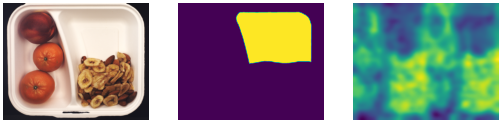
\includegraphics[width=0.45\textwidth]{figures/appendix/appendix_main_ensemble/BB/image_prediction_128.png}
        \hfill
        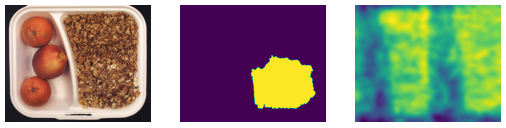
\includegraphics[width=0.45\textwidth]{figures/appendix/appendix_main_ensemble/BB/image_prediction_272.png}

    \end{subfigure}
    \begin{subfigure}[b]{\textwidth}
        \centering
        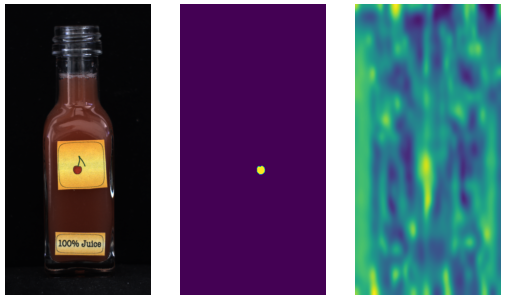
\includegraphics[width=0.45\textwidth]{figures/appendix/appendix_main_ensemble/JB/image_prediction_268.png}
        \hfill
        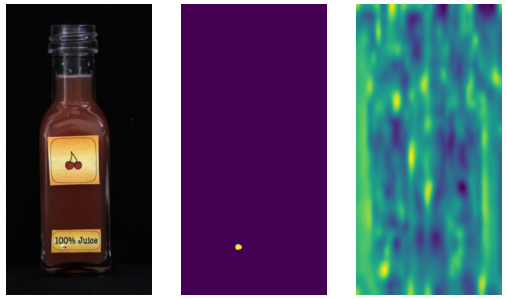
\includegraphics[width=0.45\textwidth]{figures/appendix/appendix_main_ensemble/JB/image_prediction_306.png}

    \end{subfigure}
    \begin{subfigure}[b]{\textwidth}
        \centering
        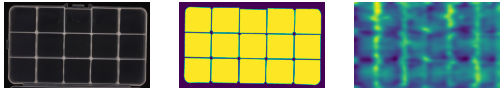
\includegraphics[width=0.45\textwidth]{figures/appendix/appendix_main_ensemble/PP/image_prediction_199.png}
        \hfill
        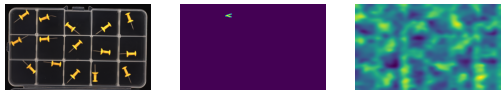
\includegraphics[width=0.45\textwidth]{figures/appendix/appendix_main_ensemble/PP/image_prediction_308.png}

    \end{subfigure}
    \begin{subfigure}[b]{\textwidth}
        \centering
        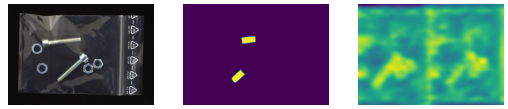
\includegraphics[width=0.45\textwidth]{figures/appendix/appendix_main_ensemble/SB/image_prediction_140.png}
        \hfill
        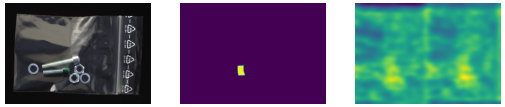
\includegraphics[width=0.45\textwidth]{figures/appendix/appendix_main_ensemble/SB/image_prediction_307.png}

    \end{subfigure}
    \begin{subfigure}[b]{\textwidth}
        \centering
        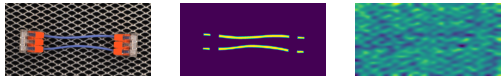
\includegraphics[width=0.45\textwidth]{figures/appendix/appendix_main_ensemble/SC/image_prediction_167.png}
        \hfill
        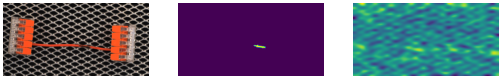
\includegraphics[width=0.45\textwidth]{figures/appendix/appendix_main_ensemble/SC/image_prediction_261.png}

    \end{subfigure}
    
    \caption{Example segmentations of the stacking ensemble approach on the MVTecAD LOCO \cite{LOCODentsAndScratchesBergmann2022} dataset.}
    \label{fig:appendixEnsemble}
\end{figure}